\chapter{Language specification}

This chapter contains an explanation on the different languages features, including code examples and a short description of the generated bytecode. For a (very) detailed description of the generated bytecode we recommend reading the source code of the \code{otld.otld.jvm.BytecodeCompiler} class as all bytecode instructions are very well documented using inline comments.

\section{Layout of a program}

Defining a program in \shortname is like defining a program in Pascal, only in \shortname you are defining a \emph{city}. A city can be defined with the command \code{City <name>;}, where \code{<name>} is replaced with the name of the program.

\subsection{City blocks}

A city consists of a number of blocks, each containing integral parts of the program. Each block starts with the statement \code{Begin <block>;} and ends with \code{End <block>;}. Each block should only occur once, and must be used in the order below. Only the \code{company} block is required.

\begin{itemize}
\item \code{depot}: This block should contain all wagons and trains.
\item \code{track}: This block should contain all signals and waypoints.
\item \code{industry}: This block should contain all factories of the city.
\item \code{company}: This block should contain the program itself.
\end{itemize}

\begin{figure}[t]
\centering
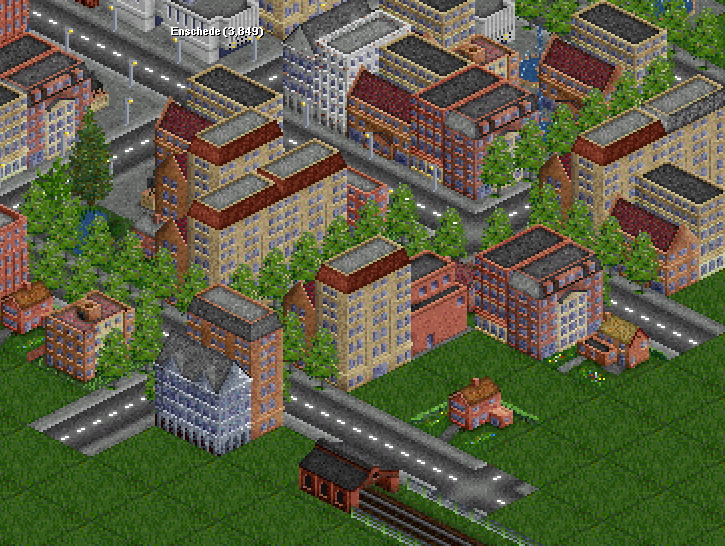
\includegraphics[scale=0.25]{Images/city_and_depot}
\caption{City and depot}
\label{fig:city_and_depot}
\end{figure}

\subsubsection*{Example}

\begin{lstlisting}
Begin depot;
	Wagon w accepts int;
End depot;

Begin track;
	Signal s is red;
	
	Waypoint p;
	Begin waypoint;
		Switch signal p;
	End waypoint;
End track;

Begin industry;
	Factory printInt accepts int produces int;
	Begin production;
		Write "Integer " platform1 to journal;
		Final product platform1;
	End production;
End industry;

Begin company;
	Load 10 into wagon w;
	Begin circle p;
		Transport w to factory printInt and fully load w;
	End circle;
End company;
\end{lstlisting}

\subsubsection*{Bytecode}

A city generates a class, constructor and main method. The constructor sets default values for the fields (see below). The main method instantiates a new object of the created class and contains the code from the \code{company} block.

\section{Basic expressions}

\subsection{Constants}

Constants can not be declared as such. However, they can be used in the program, for example in assignments. The list below contains the available types with a regex showing the valid inputs.

Strings cannot be used in variables, but are only included for in- and outputs.

\begin{itemize}
\item Integer: \verb=-?(0|[1-9][0-9]*)=
\item Boolean: \verb=red|green= (where \verb|red| is false and \verb|green| is true)
\item Character: \verb='[a-zA-Z0-9]'=
\item String: \verb="~["]*(""~["]*)*"=
\end{itemize}

\subsubsection*{Bytecode}

String constants are loaded on the stack using \code{ldc}. The other values are built from an integer using \code{biload} and math operations.

\subsection{Variable declarations}

Variables in \shortname are called \emph{wagons}. Wagons are statically typed. The type should be set on declaration.
A wagon can be declared with the statement \code{Wagon <id> accepts <type>;} where \code{<id>} is a unique identifier for the wagon and \code{<type>} is the type of the wagon. Variables can only be declared in the \code{depot} city block.

Booleans can also be stored in a \emph{signal}. The declaration and assignment of signals is different from wagons. A signal can be declared with the statement \code{Signal <id> is <color>;} where \code{<color>} is either \code{red} or \code{green}. Signals are used with conditionals. Signals can only be declared in the \code{track} city block.

The indentifiers of wagons and signals must be unique for all wagons and signals. In other words, there cannot be a wagon and a signal which share a name. Furthermore, the identifiers cannot start with the string \code{platform} since this is a reserved name.

\subsubsection*{Example}

\begin{lstlisting}
Wagon w1 accepts int;
Wagon w2 accepts boolean;
Signal s is green;
\end{lstlisting}

\subsubsection*{Bytecode}

Wagons and signals are added as fields to the generated class. Standard primitive types are used.

\subsection{Assignment}

A constant value or a value from another variable can be assigned to a variable.

To assign a constant to a variable use the statement \code{Load <const> into wagon <id>;} where \code{<const>} is the constant and \code{<id>} is the identifier for the wagon.

To copy the value of an existing wagon into another wagon use \code{Transfer wagon <id> to wagon <id>;}. The term `transfer' does not mean that the source wagon will be empty -- it remains untouched.

\subsubsection*{Example}

\begin{lstlisting}
Load 10 into wagon w1;
Load red into wagon w2;
Transfer wagon w1 into wagon w3;
\end{lstlisting}

\subsubsection*{Bytecode}

For variable assignments, the value of a field is loaded on the stack and directly stored in another field. For value assignments, the constant is loaded on the stack and stored in the field.

\subsection{Arithmetic operations}

There are two unary operations with each a special syntax:

\begin{itemize}
\item Unary minus: Inverts a wagon (integer, boolean). \\ \code{Turn wagon <id> around;}
\item Not (for signals): Inverts a signal. \\ \code{Switch signal <id>;}
\end{itemize}

The other operations use the statement \code{Transport <id>, <id> to factory <op> and fully load <id>;}. The first to occurances of \code{<id>} are the left- and righthand variables for the operation, the third \code{<id>} is the destination wagon. The operation \code{<op>} can be any of the following:

\begin{itemize}
\item Addition: \code{add} (integer, integer $\to$ integer)
\item Subtraction: \code{subtract} (integer, integer $\to$ integer)
\item Multiplication: \code{multiply} (integer, integer $\to$ integer)
\item Division: \code{divide} (integer, integer $\to$ integer)
\item Modulo division: \code{modulo} (integer, integer $\to$ integer)
\item Less than: \code{complt} (any, any $\to$ boolean)
\item Greater than: \code{compgt} (any, any $\to$ boolean)
\item Less than or equal: \code{complte} (any, any $\to$ boolean)
\item Greater than or equal: \code{compgte} (any, any $\to$ boolean)
\item Equal: \code{compeq} (any, any $\to$ boolean)
\item Logical and: \code{and} (bool|int, bool|int $\to$ bool|int)
\item Logical or: \code{or} (bool|int, bool|int $\to$ bool|int)
\end{itemize}

The operations that return a boolean can be used in two ways; either as mentioned above or with the statement \code{Transport <id>, <id> to factory <op> and set signal <id>;} to store the boolean in a signal.

\subsubsection*{Example}

\begin{lstlisting}
Turn wagon w1 around;
Transport w1, w2 to factory multiply and fully load w1;
Transport w1, w2 to factory complt and set signal s2;
Transport s1, s2 to factory and and set signal s1;
Switch signal s1;
\end{lstlisting}

\subsubsection*{Bytecode}

In all cases the values are loaded on the stack first. Then, the specific operation is executed.

For mathematical operations this is simply a bytecode instruction. For comparisons, the second value is subtracted from the first. Then, the appropriate bytecode instruction is used. Labels make sure that either a 1 (for true) or 0 (for false) is put on the stack.

\section{Block statments}

\subsection{Conditionals (if/else)}

Conditional statements are based on signals. A conditional statement starts with \code{Approach signal <id>;} where \code{<id>} is the signal that indicates which path to choose. Code under \code{Case green;} is executed when the signal is green, code under \code{Case red;} is executed when the signal is red. The statement ends with \code{Pass signal;}.

The \code{Case} statements are not required, these just function as the start points for each block. The code under these statements is executed up until another \code{Case} statement or \code{Pass signal}. Multiple case statements for the same boolean value are allowed, however, the code of a second statement will just be appended to the code from the first.

\subsubsection*{Example}

\begin{lstlisting}
Approach signal s;
	Case red:
		Write "Train delayed: " s to journal;
Pass signal;
\end{lstlisting}

\subsubsection*{Bytecode}

Since our conditionals work with boolean variables instead of inlined condition expressions, the bytecode is very simple. The boolean value is put on the stack, then \code{ifne} is executed, since ``not equal to zero'' means that the boolean is true. Labels make sure that only the part for `true' or `false' is executed.

\subsection{Loops (while)}

In \shortname \emph{circles} can be used for loops. Before defining the loop itself, the loop condition (\emph{waypoint}) needs to be defined. A waypoint can be defined with \code{Waypoint <id>;}. A waypoint behaves exactly the same way as a signal, but with one difference. It is possible to programmatically define the value of the waypoint every time it is accessed. To do this, add a waypoint block directly after the waypoint (\code{Begin waypoint;} and \code{End waypoint;}). Code in this waypoint block should write a boolean value to the identifier of the waypoint. Waypoints can only be declared in the \code{track} city block.

The code that should be executed in each iteration should be in a circle block starting with \code{Begin circle <id>;} and ending with \code{End circle;} where \code{<id>} is the identifier of the waypoint. To break out of a circle the statement \code{Stop;} can be used.

Since waypoints are a special case of signals, all normal operations for signals can be used with waypoints.

\begin{figure}[t]
\centering
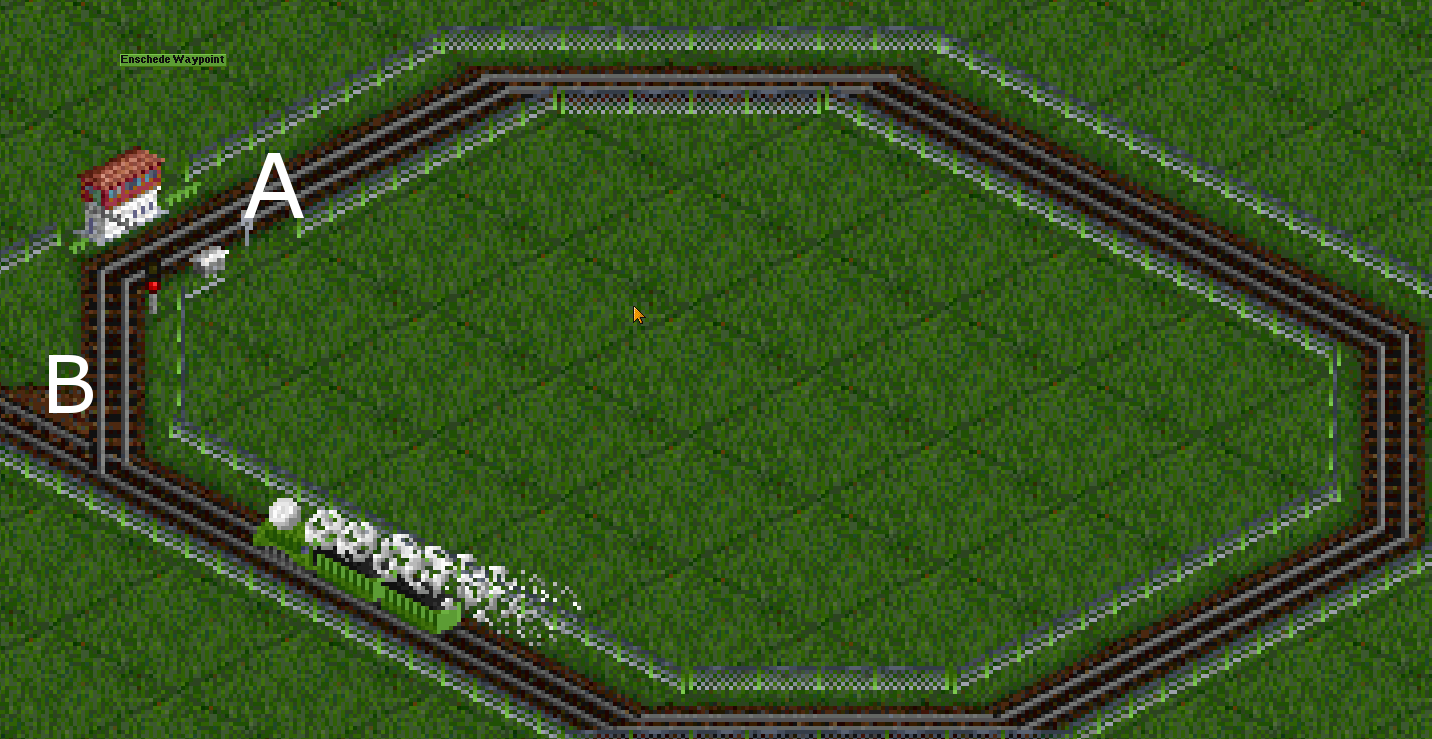
\includegraphics[scale=0.25]{Images/circle}
\caption{Circle with waypoint (\code{A} represents the circle, \code{B} is the waypoint/condition)}
\label{fig:circle}
\end{figure}

\subsubsection*{Example}

\begin{lstlisting}
Waypoint p;
Begin waypoint;
	Transport i, length to factory complt and set signal p;
	Switch signal p;
End waypoint;

Begin circle p;
	Write "This is executed a single time: " p to journal;
	Stop;
	Write "This is not executed: " p to journal;
End circle;
\end{lstlisting}

\subsubsection*{Bytecode}

A loop has a condition body (the \code{waypoint} block) and the real body (the \code{circle} block). A loop starts with the condition label, then the condition body. The boolean condition is checked the same way as with a condition. At the end of the real body a jump back to the condition is added. A break adds a jump to the end of the loop.

\subsection{Functions}

Functions are represented as \emph{factories}. Factories can be defined in the \code{industry} city block using the statement \code{Factory <id> accepts <type>[, <type>]* produces <type>;}, where \code{<id>} is the name of the factory and \code{<type>} is one of the supported variable types. This statement should be directly followed by a \code{production} block for the body of the function. This block should always end with \code{Final product <var>;}, which returns \code{<var>}. Returns are only allowed at this spot. The arguments can be accessed in the function body using \code{platformX} as variable name, where \code{X} is the 1-indexed argument index.

A function can be called similarly to an arithmetic operation with the \code{Transport <id>, <id> to factory <op> and fully load <id>;} statement where \code{<op>} is the factory name.

\begin{figure}[t]
\centering
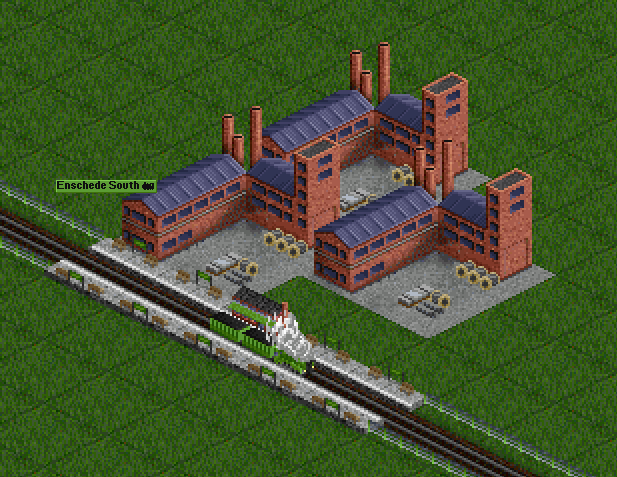
\includegraphics[scale=0.25]{Images/factory}
\caption{Factory}
\label{fig:factory}
\end{figure}

\subsubsection*{Example}

\begin{lstlisting}
Factory isZero accepts int produces boolean;
Begin production;
	Load 0 into wagon zero;
	Transport platform1, zero to factory eq and fully load temp;
	Final product temp;
End production;

Transport w1 to factory half and set signal s1;
\end{lstlisting}

\subsubsection*{Bytecode}

Functions are added as methods to the class.

Function calls generate a \code{invokevirtual} on the instance of the generated class.

\subsection{Input and output}

The program can receive input from the user (stdin) and output values (stdout).

To receive input, use \code{Ask control <question> about contents of <id>;} to ask the user to input a value for a wagon with \code{<id>} as identifier. For signals, the statement is \code{Ask control <question> about status of <id>;}. \code{<question>} is in both cases a string which is used as prompt.

To write a value to the standard output, use \code{Write <info> <id> to journal;}, where \code{<info>} is a string containing information about the value and \code{<id>} is the wagon or signal to print.

\subsubsection*{Example}

\begin{lstlisting}
Ask control "Set signal " about status of s;
Write "Signal set to " s to journal;
\end{lstlisting}

\subsubsection*{Bytecode}

For input, a new \code{Scanner} object is constructed using \code{invokespecial} and \code{getstatic} on \code{System} (for \code{System.in}). For each type of variable the appropriate method is called (\code{nextInt()}, \code{nextBoolean()} or \code{next(".").chatAt(0)}). These methods are called using \code{invokevirtual}.

For output, \code{System.out.print} and \code{System.out.println} are called using \code{getstatic} and \code{invokevirtual}.

\subsection{Comments}

It is possible to comment source code. Only block comments are supported. The style is similar to the block comments of languages like C and Java.

\subsubsection*{Example}

\begin{lstlisting}
/* Commented with Java equivalent */
Wagon w accepts int;   /* int w; */
Load 10 into wagon w;  /* w = 10; */
\end{lstlisting}

\subsubsection*{Bytecode}

Comments are ingored by the Antlr grammar, so there is no bytecode for comments.
